\chapter{Kräfte, Quarks und die ersten Hadronmultipletts}

\section{Teilchen, Felder und das fehlende dritte Element}

Wellen sind Feldkonfigurationen, daher hängen die beiden Beschreibungen in der vorliegenden Diskussion eng zusammen. Die Quantenmechanik besagt, dass die Energie einer solchen Welle in diskreten, unteilbaren Einheiten auftritt. Diese Einheiten sind ihre Quanten; die Quanten eines Feldes nennen wir seine Teilchen. Mit diesem Zusammenhang haben wir bereits Wellengleichungen, Wirkungsprinzipien und die grundlegenden Eigenschaften von Teilchen besprochen: Energie, Impuls, Spin und die Unterscheidung zwischen Bosonen--und Fermionen. Fermionen widersetzen sich der Besetzung desselben Zustands; Bosonen können sich in einem Zustand ansammeln und kondensieren.

Eine Quanten-Lagrangedichte erfasst auch Wechselwirkungen. Produkte von Feldern stellen Vertizes dar, an denen Teilchen ein- und ausgehen. Ein Term mit vier Feldfaktoren etwa beschreibt einen Wechselwirkungsvertex mit vier Beinen. So wird das Wirkungsprinzip zu einem kompakten Verzeichnis möglicher Teilchenprozesse.

Als Nächstes müssen wir die Teilchen benennen---nicht ganz einzeln, sondern in Familien---und jedem eine gewisse Eigenart zuschreiben: seine Eigenschaften, Wechselwirkungen und seinen Platz in der gewöhnlichen Physik. Bevor wir diese Liste aufstellen, fehlt jedoch noch eine Seite eines begrifflichen Dreiecks:
\begin{itemize}
\item Teilchen,
\item Felder, deren Quanten diese Teilchen sind,
\item Kräfte, die mit Austauschprozessen unter Beteiligung eben dieser Quanten verbunden sind.
\end{itemize}

Das Wort \emph{elementar} muss vorläufig bleiben. Jede plausible Definition eines elementaren Teilchens im Gegensatz zu einem zusammengesetzten stößt früher oder später auf einen schwer fassbaren Grenzfall; auf dieses Problem kommen wir zurück. Nehmen wir zunächst an, dass es fundamentale Felder gibt, und nennen wir deren Quanten Elementarteilchen. Wenn ein elektrisches Feld elektrische Kräfte hervorruft und ein Gravitationsfeld Gravitationskräfte, dann muss auch das Elektronenfeld an Kräften beteiligt sein. Das Dreieck schließt sich nur, wenn sich Kräfte neben der Feldbeschreibung auch durch Teilchen beschreiben lassen.

Wir werden die Logik der Kraft daher auf zwei Wegen herleiten. Zunächst verwenden wir die Energie klassischer Felder; anschließend fragen wir, wie dieselbe Wechselwirkung erscheint, wenn man ein Feld in seine Quanten auflöst. Erst wenn diese Verbindung hergestellt ist, beginnen wir mit dem Teilchenkatalog.

\section{Kraft aus Feldenergie in der klassischen Elektrodynamik}

Man bringe zwei Ladungen im Raum an. Eine Möglichkeit, ihre Kraft zu bestimmen, besteht darin, das Kraftgesetz mit dem umgekehrten Quadrat des Abstands anzuführen. Aufschlussreicher ist die Frage, was die Ladungen mit dem Raum machen: Sie erzeugen elektrische Felder, und diese Felder speichern Energie.

Es ist hilfreich, jede Ladung von der räumlichen Form ihres Feldes zu trennen,
\begin{equation}
\mathbf E_i=q_i\widehat{\mathbf E}_i,
\end{equation}
auch wenn wir die Hutnotation nicht beibehalten müssen. Sind beide Ladungen vorhanden, ergibt die Linearität
\begin{equation}
\mathbf{E}=\mathbf{E}_1+\mathbf{E}_2.
\end{equation}
Bis auf die Wahl der Einheiten hat die elektrostatische Feldenergie die Form
\begin{equation}
U_{\text{field}}\propto\int d^3x\,\mathbf{E}^2.
\end{equation}
Setzt man die Summe der beiden Felder ein, erhält man
\begin{align}
U_{\text{field}}
&\propto\int d^3x\,(\mathbf{E}_1+\mathbf{E}_2)^2 \\
&\propto\int d^3x\,\bigl(\mathbf{E}_1^2+\mathbf{E}_2^2
  +2\mathbf{E}_1\!\cdot\!\mathbf{E}_2\bigr).
\end{align}

Die ersten beiden Terme sind Selbstenergien. Verschiebt man eine der Ladungen, bewegt sich ihr Feld mit ihr, und das entsprechende Integral ändert sich nicht. Diese Energie trägt über \(E=mc^2\) zur gemessenen Masse des isolierten geladenen Teilchens bei. Wie diese Selbstenergie in die gemessene Masse eingeht, gehört zum späteren Thema der Renormierung. Zu der von der Position unabhängigen Energie trägt nichts zur Kraft zwischen den beiden Teilchen bei.

Beim Kreuzterm ist das anders. Er gehört keinem der Teilchen für sich allein und tritt nur auf, wenn beide Felder vorhanden sind. Sind die Ladungen sehr weit voneinander entfernt, überlappen sich die Bereiche, in denen ihre Felder nennenswert sind, kaum. Nähern sich die Ladungen, verändert sich die Überlappung. Die von der Konfiguration abhängige Wechselwirkungsenergie ist daher proportional zu
\begin{equation}
U_{\text{int}}(r)\propto q_1q_2\int d^3x\,
\widehat{\mathbf E}_1\!\cdot\!\widehat{\mathbf E}_2.
\end{equation}
Für zwei Punktladungen mit Abstand \(r\) ergibt die Auswertung des Integrals die bekannte Abhängigkeit
\begin{equation}
U_{\text{int}}(r)\propto\frac{q_1q_2}{r}.
\end{equation}
Die radiale Kraft ist ihr negativer Gradient,
\begin{equation}
\mathbf F_{12}=-\boldsymbol\nabla_{\mathbf r}U_{\text{int}},
\qquad
|\mathbf F_{12}|\propto\frac{|q_1q_2|}{r^2}.
\end{equation}
\editorialnote{In der mündlichen Herleitung wird der Kreuzterm ohne Zwischenstopp beim Potenzial mit der Coulomb-Kraft, die mit dem umgekehrten Quadrat des Abstands abnimmt, in Verbindung gebracht. Das übliche Zwischenergebnis \(U_{\mathrm{int}}\propto1/r\) ist hier ausdrücklich angegeben, damit sein Gradient die angegebene \(1/r^2\) Kraft ergibt.}

Das Kraftgesetz ist nun die Ableitung des Anteils der Feldenergie, der von der Relativlage abhängt. In großem Abstand sind die beiden Objekte praktisch unabhängig voneinander. Bringt man sie zusammen, wird das Feld zwischen ihnen umgeordnet; die daraus folgende Energieänderung ist die Wechselwirkung.

Doch wenn sich ein Feld in Quanten auflösen lässt, kann dies nicht das Ende der Geschichte sein. Für dieselbe Kraft muss es auch eine Beschreibung in Teilchensprache geben.

\section{Molekularer Austausch: zwei Protonen und ein Elektron}

Bevor wir zur Elektrodynamik zurückkehren, betrachten wir ein System, bei dem sich Austausch anschaulicher darstellen lässt: zwei Protonen und ein Elektron. Austausch ist nur eine von mehreren Ursachen molekularer Kräfte, doch dieses Beispiel macht den Zusammenhang zwischen Austausch, Energie und Kraft sichtbar. Es ist kein Ersatz für die Quantenelektrodynamik.

Ist ein Proton vorhanden und das andere unendlich weit entfernt, kann sich das Elektron im wasserstoffartigen Grundzustand befinden, der am ersten Proton zentriert ist. Seine Wellenfunktion ist in der Nähe dieses Kraftzentrums lokalisiert.

\begin{figure}[h]
\centering
\includegraphics[width=0.72\textwidth]{lecture_01_figure_02.png}

\medskip

\begin{tikzpicture}[scale=0.95]
\draw (-0.2,0) -- (6.4,0);
\fill (1.3,0) circle (2pt);
\draw[smooth] plot coordinates {(0.1,0.15) (0.8,1.15) (1.5,1.75) (2.2,1.1) (3.0,0.35) (3.8,0.12)};
\node at (1.3,-0.35) {$p$};
\node at (2.7,1.55) {$\psi_1(x)$};
\end{tikzpicture}
\caption{Eine wasserstoffartige Grundzustandswellenfunktion, lokalisiert in der Nähe eines Protons.}
\lectureframe{00:14:32}
\end{figure}
\editorialnote{Die Bezeichnung \(\psi_1(x)\) benennt in der Neuzeichnung das bei 00:14:30--00:14:32 beschriebene lokalisierte Profil; sie wurde nicht von einer lesbaren Beschriftung an der Tafel übernommen.}

Nun bringen wir ein zweites Proton in großem, aber endlichem Abstand hinzu. Aufgrund der Symmetrie gibt es einen zweiten lokalisierten Zustand mit derselben Energie wie der Ein-Zentren-Zustand, diesmal am rechten Proton zentriert.

\begin{figure}[h]
\centering
\includegraphics[width=0.78\textwidth]{lecture_01_figure_03.png}

\medskip

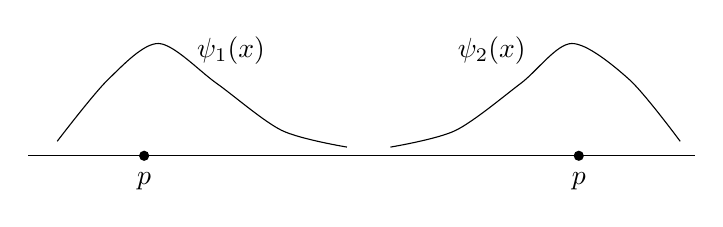
\begin{tikzpicture}[scale=0.92]
\draw (-0.2,0) -- (9.0,0);
\fill (1.4,0) circle (2pt);
\fill (7.4,0) circle (2pt);
\draw[smooth] plot coordinates {(0.2,0.2) (0.9,1.05) (1.6,1.55) (2.4,1.0) (3.3,0.35) (4.2,0.12)};
\draw[smooth] plot coordinates {(4.8,0.12) (5.7,0.35) (6.6,1.0) (7.3,1.55) (8.1,1.05) (8.8,0.2)};
\node at (1.4,-0.35) {$p$};
\node at (7.4,-0.35) {$p$};
\node at (2.6,1.45) {$\psi_1(x)$};
\node at (6.2,1.45) {$\psi_2(x)$};
\end{tikzpicture}
\caption{Die beiden lokalisierten Profile, aus denen die Gleichgewichtssuperposition gebildet wird, sobald Tunneln zugelassen ist.}
\lectureframe{00:17:54}
\end{figure}
\editorialnote{Die Bezeichnungen \(\psi_1(x)\) und \(\psi_2(x)\) kennzeichnen die beiden bei 00:17:41--00:17:56 besprochenen Profile; die Symbole sind schematische Bezeichnungen, die der besseren Lesbarkeit halber hinzugefügt wurden.}

Bei unendlichem Abstand sind die beiden Zustände entartet: Es kostet gleich viel Energie, das Elektron links oder rechts zu lokalisieren. Bei endlichem Abstand wird ein neuer Prozess möglich. Das Elektron kann durch den klassisch verbotenen Bereich von einem Zentrum zum anderen tunneln. Eine Bahn durch die Barriere zu verfolgen, würde den Zustand stören; ``Hüpfen'' beschreibt die quantenmechanische Entwicklung, nicht die Aufnahme einer klassischen Bahn.

Im Gleichgewicht ist die Wahrscheinlichkeit gleich groß, das Elektron in der Nähe des einen oder des anderen Protons zu finden. Die Normierung liefert daher den Faktor \(1/\sqrt2\), und der niedrigere Gleichgewichtszustand ist näherungsweise
\begin{equation}
\psi_+(x)\approx \frac{\psi_1(x)+\psi_2(x)}{\sqrt2}.
\end{equation}

Das Näherungszeichen ist wichtig. Die tatsächliche Wellenfunktion des Zweizentrenproblems ist nicht exakt die Summe zweier unveränderter wasserstoffartiger Orbitale; im Überlappungsbereich passt sie sich an. Entscheidend ist hier, dass der symmetrische Gleichgewichtszustand unterhalb der Energie des isolierten Ein-Zentren-Zustands liegt. In der Sprache des Hamiltonoperators sind die linke und die rechte Konfiguration durch ein außerdiagonales Matrixelement gekoppelt. Wenn das Elektron ihre kohärente Superposition einnehmen kann, sinkt die Energie.

\section{Von der abgesenkten Energie zur effektiven Kraft}

Bei großem Protonenabstand nähert sich der vom Elektron verursachte Beitrag \(E_e(r)\) seinem Wert für getrennte Atome. Bei kleinerem Abstand senken Tunneln und Superposition ihn. Das vollständige Potenzial des Zwei-Protonen--Ein-Elektron-Systems muss auch die direkte Abstoßung der Protonen enthalten,
\begin{equation}
V_{\mathrm{tot}}(r)=V_{pp}(r)+E_e(r).
\end{equation}

Damit knüpft das Molekülbeispiel wieder an die Herleitung über die Feldenergie an. Die Skizzen der Wellenfunktionen und die qualitative Kurve für \(E_e(r)\) sind zwei Ansichten derselben Rechnung; das Gleichgewicht wird durch die Summe \(V_{\mathrm{tot}}(r)\) bestimmt.

\begin{figure}[h]
\centering
\includegraphics[width=0.78\textwidth]{lecture_01_figure_04.png}

\medskip

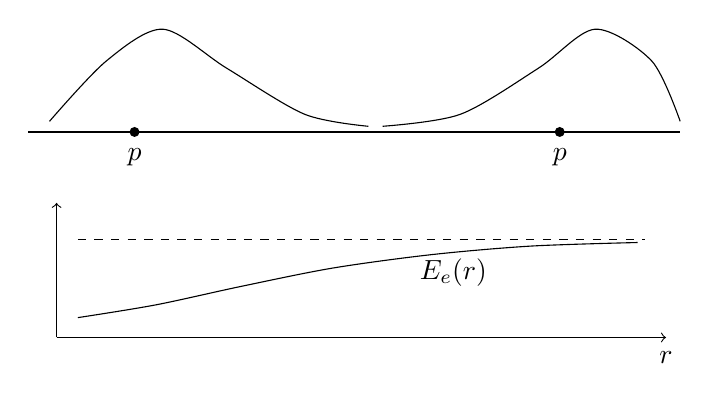
\begin{tikzpicture}[scale=0.9]
\draw (-0.2,3.0) -- (9.0,3.0);
\fill (1.3,3.0) circle (2pt);
\fill (7.3,3.0) circle (2pt);
\draw[smooth] plot coordinates {(0.1,3.15) (0.9,4.0) (1.7,4.45) (2.6,3.9) (3.7,3.25) (4.6,3.08)};
\draw[smooth] plot coordinates {(4.8,3.08) (5.9,3.25) (7.0,3.9) (7.8,4.45) (8.6,4.0) (9.0,3.15)};
\node at (1.3,2.65) {$p$};
\node at (7.3,2.65) {$p$};

\draw[->] (0.2,0.1) -- (0.2,2.0);
\draw[->] (0.2,0.1) -- (8.8,0.1);
\draw[dashed] (0.5,1.48) -- (8.5,1.48);
\draw[smooth] plot coordinates {(0.5,0.38) (1.6,0.56) (2.8,0.82) (4.1,1.08) (5.5,1.27) (6.9,1.39) (8.4,1.44)};
\node at (5.8,1.02) {$E_e(r)$};
\node at (8.8,-0.18) {$r$};
\end{tikzpicture}
\caption{Oben die Überlappung der Wellenfunktionen, darunter die vom Elektron verursachte Energie. Sie steigt bei zunehmendem \(r\) gegen den Grenzwert für getrennte Atome; das Gesamtpotenzial der Protonen muss auch ihre Coulomb-Abstoßung enthalten.}
\lectureframe{00:20:28}
\end{figure}
\editorialnote{Die Bezeichnungen \(E_e(r)\) und \(r\) kennzeichnen die bei 00:19:12--00:20:38 besprochene Energiekurve und den Abstand; im erhaltenen Tafelbild sind diese Achsenbeschriftungen nicht lesbar.}

Die beiden zugehörigen Kräfte ergeben sich aus den Energiegradienten,
\begin{equation}
F_{e}(r)=-\frac{dE_e}{dr},
\qquad
F_{\mathrm{tot}}(r)=-\frac{dV_{\mathrm{tot}}}{dr}.
\end{equation}
Das System wird also zu niedrigerer Gesamtenergie gedrängt. Wo \(E_e(r)\) abnimmt, wenn sich die Protonen nähern, liefert der Austausch einen anziehenden Beitrag; ob ein gebundener Abstand existiert, hängt davon ab, wie dieser Beitrag mit \(V_{pp}(r)\) konkurriert. Das ist der grundlegende Mechanismus hinter einer kovalenten Bindung: Das Elektron wird gemeinsam genutzt, weil der gemeinsame Zustand energetisch günstig ist.

In der klassischen Rechnung verändert die Überlappung elektrischer Felder die Energie. Hier ermöglichen zwei Kraftzentren einen Zustand niedrigerer Quantenenergie. Beide Mechanismen erzeugen eine Kraft, weil die Gleichgewichtsenergie von der Konfiguration abhängt.

Die Sprache des Austauschs lässt sich durch eine Skizze von Weltlinien zusammenfassen. Sie darf nicht als beobachtete Bahn gelesen werden, sondern stellt Amplituden dafür dar, dass das Elektron dem einen oder dem anderen Proton zugeordnet ist.

\begin{figure}[h]
\centering
\begin{tikzpicture}[scale=1.0]
\draw (0,0) -- (0,4.4);
\draw (4.8,0) -- (4.8,4.4);
\draw (0,0.9) .. controls (1.6,1.7) and (3.2,1.7) .. (4.8,2.5);
\draw (4.8,2.9) .. controls (3.2,2.1) and (1.6,2.1) .. (0,3.9);
\node at (0,-0.35) {$p$};
\node at (4.8,-0.35) {$p$};
\node at (2.35,1.55) {$e^-$};
\node at (2.35,2.55) {$e^-$};
\end{tikzpicture}
\caption{Elektronenaustausch zwischen zwei Protonen-Weltlinien, als schematische Darstellung von Quantenamplituden und nicht einer beobachteten Bahn zu verstehen.}
\end{figure}

\begin{classroomqa}
\audiencequestion{Lässt sich die Anziehung einfach dadurch erklären, dass das Elektron die Protonenladung abschirmt oder verringert?\lecturetimestamp{00:23:26}}
\lecturerresponse{Nein. Eine Verringerung der Ladung ist keine passende Vorstellung für diesen Effekt. Entscheidend ist, dass die Summe der beiden lokalisierten Wellenfunktionen einen Zustand ergibt, dessen Energie geringfügig niedriger ist als die jedes der beiden lokalisierten Zustände für sich.}
\end{classroomqa}

\begin{classroomqa}
\audiencequestion{Ist das gemeint, wenn Feynman sagte, ``Licht möge Licht''?\lecturetimestamp{00:23:51}}
\lecturerresponse{Nein. Mit dieser Formulierung ist wahrscheinlich die Bose-Statistik gemeint: Photonen bevorzugen gemeinsame Zustände, während Elektronen dem Ausschlussprinzip gehorchen. Der molekulare Effekt hier beruht auf Tunneln zwischen zwei Zentren.}
\end{classroomqa}

Die beiden Protonen stoßen sich weiterhin elektrostatisch ab. Der Austausch ist kurzreichweitiger als die Coulomb-Wechselwirkung; daher muss man das Gesamtpotenzial betrachten und nicht nur einen der beiden Beiträge. Bei passenden Abständen ist das Molekülion \(\mathrm H_2^+\) dennoch gebunden; in einem neutralen System mit zwei Elektronen fehlt die langreichweitige Ladungsabstoßung, und kovalente Bindung ist noch vertrauter.

\begin{classroomqa}
\audiencequestion{Verringert das Elektron zwischen den Protonen hauptsächlich ihre elektrostatische Abstoßung?\lecturetimestamp{00:24:33}}
\lecturerresponse{Es verringert die Abstoßung ein wenig, doch das ist nicht der Haupteffekt. Elektronenaustausch ist eine kurzreichweitigere Kraft als die Coulomb-Abstoßung. Am deutlichsten zeigt er sich in einem neutralen System mit zwei Elektronen: Dort fehlt die langreichweitige elektrostatische Kraft zwischen den Atomen, doch Tunneln erzeugt weiterhin eine Anziehung.}
\end{classroomqa}

\begin{classroomqa}
\audiencequestion{Ist das positiv geladene Molekülion \(\mathrm H_2^+\) mit nur einem Elektron tatsächlich gebunden?\lecturetimestamp{00:26:06}}
\lecturerresponse{Ja. Bei hinreichend kleinem Abstand ist die Austauschanziehung stark genug, um die Coulomb-Abstoßung zwischen den Protonen zu überwinden.--}
\end{classroomqa}

\begin{classroomqa}
\audiencequestion{Erzeugt die Anordnung mit zwei Zentren eine dritte Kraft?\lecturetimestamp{00:26:24}}
\lecturerresponse{Es wird keine neue fundamentale Kraft eingeführt. Die Schr\"odingerGleichung im Gesamtpotenzial der beiden Protonen hat eine andere Gleichgewichtsenergie als das Ein-Zentren-Problem; die Ableitung dieser veränderten Energie ist die effektive Kraft.}
\end{classroomqa}

\begin{classroomqa}
\audiencequestion{Ist die Energieabsenkung ein Beispiel für Quantenverschränkung?\lecturetimestamp{00:27:06}}
\lecturerresponse{Nicht im üblichen Sinn für zwei Teilchen: Es wird nur ein Elektron benötigt. Das relevante mathematische Merkmal ist ein außerdiagonales Matrixelement des Hamiltonoperators, das den linken und den rechten Zustand koppelt.}
\end{classroomqa}

\begin{classroomqa}
\audiencequestion{Was geschieht bei hoher Temperatur mit dem Austausch?\lecturetimestamp{00:27:37}}
\lecturerresponse{Bei extrem hoher Temperatur wird das Elektron ionisiert und löst sich ganz vom Molekül. Bei geringerer Anregungsenergie kann es ein größeres Orbital besetzen, wodurch sich die Überlappung und damit die Kraft ändern. Das ist eine zustandsabhängige Korrektur und kein neuer allgemeiner Mechanismus.}
\end{classroomqa}

\section{Photonenaustausch und die ersten Einträge der Tabelle}

Lässt sich die Coulomb-Kraft ebenso in der Sprache des Austauschs beschreiben? Ein geladenes Teilchen wechselwirkt mit dem elektromagnetischen Feld, dessen Quanten Photonen sind. Klassisch lösen wir das elektrische Feld um die Ladung herum. In der Quantenfeldtheorie zerlegen wir diese Wechselwirkung in Photonemission und -absorption.

Ein physikalisches geladenes Teilchen ist nicht einfach eine nackte Ladung. Sein Zustand ist eine quantenmechanische Superposition, die einen Anteil mit einem nackten Elektron, ein Elektron mit einem Photon, ein Elektron mit zwei Photonen und so weiter enthält. In bewusst schematischer Schreibweise:
\begin{equation}
\begin{aligned}
\ket{e_{\mathrm{phys}}}
={}&a_0\ket e
+a_1\ket{e+\text{one photon}}
\\
&+a_2\ket{e+\text{two photons}}+\cdots .
\end{aligned}
\end{equation}
Diese Schreibweise gibt lediglich die Hierarchie der Photonenzahlanteile an; sie legt weder die Photonenimpulse fest noch versucht sie, einen wechselwirkenden geladenen Zustand vollständig zu konstruieren.
Die umgebenden Photonen werden emittiert und wieder absorbiert, statt als freie Strahlung zu entkommen. Ihre Auswirkungen lassen sich messen, obwohl sie nicht auf dieselbe Weise wie frei propagierende Photonen nachgewiesen werden. Bringt man eine zweite Ladung in die Nähe, kann ein an der einen Ladung emittiertes Photon an der anderen absorbiert werden. Die Energien der beiden bekleideten Zustände sind dann nicht mehr einfach die Summe zweier isolierter Energien.

Als Anschauungsbild kann man sich zwei Jongleure vorstellen, die jeweils mit mehreren Bällen hantieren. Sind sie weit voneinander entfernt, jongliert jeder für sich. Kommen sie nahe genug zusammen, kann einer einen Ball fangen, den der andere geworfen hat. In der Sprache der Feynman-Diagramme ist dieses gemeinsame Objekt das ausgetauschte Photon. Die Analogie beschreibt keine mikroskopische Bahn, macht aber deutlich, warum die Nähe einen neuen Prozess ermöglicht.

Nun haben wir zwei Beschreibungen, die über das bloße Auswendiglernen des Coulomb-Gesetzes hinausgehen. In der klassischen Feldtheorie addiert man die Felder und quadriert das Ergebnis. In der Quantenfeldtheorie summiert man Amplituden, bei denen Quanten ausgetauscht werden. In diesem Sinn besteht eine Eins-zu-eins-zu-eins-Zuordnung zwischen Teilchen, Feldern und Kräften. Elektronen vermitteln molekularen Austausch, Photonen elektromagnetischen Austausch, und jedes Teilchen, das ausgetauscht werden kann, kann in einem geeigneten Zusammenhang zu einer Kraft beitragen. Die vertraute Aussage, die Natur habe vier fundamentale Wechselwirkungen, ist also eine Klassifikation auf einer allgemeineren Ebene; in der Sprache des Austauschs kann jede austauschbare Teilchensorte einen eigenen effektiven Kraftbeitrag erzeugen.

Nun ist es endlich an der Zeit, die Teilchen zu benennen, ihre Eigenschaften aufzulisten und anzugeben, an welchen Prozessen sie teilnehmen können. Das gesamte Standardmodell auf einmal aufzuschreiben, wäre nur ein langer Gedächtnistest. Deshalb teilen wir die Teilchen in kleine Gruppen mit einfachen Zusammenhängen zwischen ihren Mitgliedern ein und lernen, was jede Gruppe kann.

Der vollständige Katalog ist unhandlich, weil wir nicht verstehen, warum genau diese Teilchen existieren und andere vorstellbare Teilchen nicht. Die mathematische Konsistenz gibt einige Zusammenhänge vor: Sobald mehrere Mitglieder eines Musters existieren, kann ein weiteres erforderlich sein, um es zu vervollständigen. Diese Zusammenhänge verringern die Zahl unabhängiger Fakten, aber nur in bescheidenem Maß. Viele Teilchentypen und zahlreiche Parameter bleiben unerklärt. Um zu verstehen, wonach spätere Experimente suchen, müssen wir diese unvollständige Struktur begreifen.

\begin{figure}[h]
\centering
\includegraphics[width=0.7\textwidth]{lecture_01_figure_05.png}
\caption{Der erste Eintrag der Teilchentabelle kennzeichnet das Photon durch \(\gamma\) und sein Feld durch das Vektorpotenzial \(A\).}
\lectureframe{00:39:11}
\end{figure}

Die erste Feld--Quanten-Zuordnung lautet
\begin{equation}
\gamma \leftrightarrow A.
\end{equation}
Dabei ist \(A\) das elektromagnetische Vektorpotenzial. Das Photon ist ein Boson mit Spin eins, elektrischer Ladung null, Baryonenzahl null und verschwindender Ruhemasse. Das Elektronenfeld wird üblicherweise mit \(\psi_e\) bezeichnet; seine Erzeugungs- und Vernichtungsanteile wirken auf Elektronen- und Positronenzustände.

Unsere Tabelle enthält den Namen, das Teilchensymbol, das Feld, den Typ als Boson oder Fermion, die elektrische Ladung \(Q\), die Baryonenzahl \(B\) und die Masse:

\begin{table}[h]
\centering
\resizebox{\linewidth}{!}{%
\begin{tabular}{lllllll}
Name & Symbol & Feld & Typ & \(Q\) & \(B\) & Masse \\
Photon & \(\gamma\) & \(A\) & Boson & \(0\) & \(0\) & \(0\) \\
Elektron & \(e^-\) & \(\psi_e\) & Fermion & \(-1\) & \(0\) & \(0.51\,\mathrm{MeV}\) \\
Positron & \(e^+\) & \(\psi_e\) & Fermion & \(+1\) & \(0\) & \(0.51\,\mathrm{MeV}\)
\end{tabular}
}%
\caption{Die Einträge für Photon und Elektron--Positron am Anfang des Teilchenkatalogs.}
\end{table}

Elektron und Positron stehen in wechselseitiger Beziehung: Jedes ist das Antiteilchen des anderen. Den negativ geladenen Zustand als ``das Teilchen'' zu bezeichnen, ist Konvention. Wir messen die elektrische Ladung in Einheiten des Betrags der Elektronenladung, also gilt
\begin{equation}
Q(e^-)=-1,\qquad Q(e^+)=+1.
\end{equation}
Die Masse wird mithilfe von \(E=mc^2\) in Energieeinheiten angegeben. Ein Elektronenvolt ist die Energie, die eine Ladung \(e\) bei einer Potenzialdifferenz von einem Volt gewinnt,
\begin{equation}
1\,\mathrm{eV}=e\,(1\,\mathrm V).
\end{equation}
Diese Einheit ergibt sich ganz natürlich aus der Atomphysik: Als grobe atomare Energieskala kostet die Ionisierung von Wasserstoff etwa \(13.5\,\mathrm{eV}\). Teilchenmassen erfordern Millionen oder Milliarden Elektronenvolt. Die Elektronenmasse beträgt
\begin{equation}
m_e c^2 \approx 0.511\,\mathrm{MeV}.
\end{equation}

\begin{classroomqa}
\audiencequestion{Müsste die Elektronenmasse genau ein halbes MeV betragen?\lecturetimestamp{00:44:02}}
\lecturerresponse{Nein. Der bequeme gerundete Wert \(0.51\,\mathrm{MeV}\) ist durch kein Prinzip auf exakt eine Hälfte festgelegt; er ist ein Messparameter.}
\end{classroomqa}

Der elementare QED-Prozess hat eine einlaufende geladene Fermionenlinie, eine auslaufende und eine daran angeschlossene Photonenlinie. Durch Umordnen oder Kreuzen der Beine kann derselbe Vertex Photonemission, -absorption oder einen Positronenprozess beschreiben. In der hier verwendeten nichtkovarianten schematischen Schreibweise enthält die Wechselwirkung
\begin{equation}
\mathcal{L}_{\mathrm{int}}\sim e\,\psi_e^\dagger \psi_e A.
\end{equation}
Entwickelt man die Felder nach Erzeugungs- und Vernichtungsoperatoren, entstehen Terme, die ein einlaufendes Elektron vernichten, ein auslaufendes Elektron erzeugen und ein Photon erzeugen oder vernichten. Die Kopplung \(e\) liefert am Vertex einen Faktor. Bei der Photonemission während der Streuung oder Beschleunigung eines Elektrons gilt daher
\begin{equation}
\mathcal{A}_{\mathrm{vertex}}\propto e,
\qquad
P_{\mathrm{emission}}\propto e^2.
\end{equation}
Ein Elektron, das auf das Target einer Röntgenröhre trifft, ist ein praktisches Beispiel, bei dem diese Photonemissionswahrscheinlichkeit eine Rolle spielt. Wiederholte Kombinationen desselben Vertex erzeugen die Prozesse der Quantenelektrodynamik, einschließlich der Energieverschiebung, die als Kraft zwischen Ladungen gedeutet wird.

Ein schematischer Vertex ist daher nützlich.

\begin{figure}[h]
\centering
\begin{tikzpicture}[scale=1.0]
\fill (0,0) circle (1.5pt);
\draw (-1.6,-1.2) -- (0,0) -- (1.6,-1.2);
\draw (0,0) -- (0,1.8);
\node at (-1.8,-1.4) {$e^-$};
\node at (1.8,-1.4) {$e^-$};
\node at (0.35,1.95) {$\gamma$};
\end{tikzpicture}
\caption{Topologisches Schema des elementaren QED-Vertices: Eine Linie eines geladenen Fermions läuft hinein, eine weitere hinaus, und ein Photon ist angekoppelt. Der gerade Photonenzweig ist hier lediglich eine vereinfachte Konvention der Darstellung.}
\end{figure}

Der Austauschbeitrag zur Kraft verbindet zwei solcher Vertizes:

\begin{figure}[h]
\centering
\begin{tikzpicture}[scale=1.0]
\draw (0,0) -- (0,4.0);
\draw (4.8,0) -- (4.8,4.0);
\draw (0,2.0) -- (4.8,2.0);
\node at (0,-0.35) {$e^-$};
\node at (4.8,-0.35) {$e^-$};
\node at (2.4,2.3) {$\gamma$};
\end{tikzpicture}
\caption{Topologisches Schema des Photonaustauschs als quantenfeldtheoretische Beschreibung der Coulomb-Wechselwirkung.}
\end{figure}

Nachdem das Dreieck aus Teilchen--Feld--Kraft geschlossen ist, können wir den Katalog fortsetzen.

\section{Quarks, Baryonenzahl und das Rätsel der Familien}

Wäre dieser Katalog um 1960 verfasst worden, wären auf Elektronen und Photonen wahrscheinlich Protonen und Neutronen gefolgt. In der modernen Teilchenphysik werden zunächst Quarks eingeführt. Im naiven Konstituentenbild sind Protonen und Neutronen vergleichsweise große zusammengesetzte Teilchen, die aus kleineren Quark-Freiheitsgraden bestehen. Was genau \emph{zusammengesetzt} bedeutet, muss noch untersucht werden; die Sprache der Konstituenten ist jedoch bereits äußerst nützlich.

Alle Quarks sind Fermionen. Sie tragen Baryonenzahl, eine Größe, die in der Kernphysik durch das Zählen der Nukleonen eingeführt wurde. Ein \emph{Nukleon} ist speziell ein Proton oder ein Neutron. \emph{Baryon} bezeichnet die umfassendere Klasse, zu der Nukleonen und die ähnlichen schweren Teilchen gehören, denen wir später begegnen. Ein Proton und ein Neutron haben jeweils eine Einheit,
\begin{equation}
B(p)=B(n)=1,
\qquad
B(\bar p)=B(\bar n)=-1.
\end{equation}
Bei einem Atomkern entspricht diese Baryonenzahl genau der Massenzahl \(A=Z+N\), also der Anzahl der Protonen plus Neutronen. Die in atomaren Masseneinheiten gemessene numerische Atommasse entspricht \(A\) nur näherungsweise. Protonen können bei Betaprozessen in Neutronen und Neutronen in Protonen umgewandelt werden, doch die Gesamtzahl der Nukleonen bleibt unverändert. Zum Beispiel
\begin{equation}
n\longrightarrow p+e^-+\bar\nu_e
\end{equation}
ändert die Anzahl der Protonen und Neutronen jeweils für sich, erhält aber ihre Summe.

\begin{classroomqa}
\audiencequestion{Widersprechen Isotope der Erhaltung der Summe aus Protonen- und Neutronenzahl?\lecturetimestamp{00:52:03}}
\lecturerresponse{Verschiedene Isotope haben tatsächlich unterschiedliche Neutronenzahlen, und beim Betazerfall können ein Neutron und ein Proton ineinander umgewandelt werden. Bei gewöhnlichen Kernprozessen ist die erhaltene Größe die Gesamtbaryonenzahl, nicht die Zahl der Teilchen einer der beiden Arten für sich.}
\end{classroomqa}

Die Normierung ist Konvention. Wir hätten einem Proton die Baryonenzahl \(2\), \(7\) oder \(\pi\) zuweisen können, sofern alle zusammengesetzten Teilchen entsprechend skaliert würden. Sobald dem Proton \(B=1\) zugewiesen ist und es aus drei Quarks besteht, muss jedes Quark die Baryonenzahl
\begin{equation}
B(q)=\frac13,
\qquad
B(\bar q)=-\frac13.
\end{equation}
tragen. Der Bruchteil ergibt sich somit historisch daraus, dass zuerst das zusammengesetzte Nukleon normiert wurde.

\begin{classroomqa}
\audiencequestion{Ist die Zahl der Quarks erhalten?\lecturetimestamp{00:54:23}}
\lecturerresponse{Quark--Antiquark-Paare können erzeugt oder vernichtet werden; die bloße Anzahl ist also nicht erhalten. Die der Baryonenzahl entsprechende Größe ist die Zahl der Quarks minus der Zahl der Antiquarks, geteilt durch drei. Empirisch ist sie mit äußerst hoher Genauigkeit erhalten, auch wenn wir hier nicht voraussetzen, dass dies ein ausnahmsloses Gesetz ist.}
\end{classroomqa}

Ein hypothetischer ladungserhaltender Zerfall wie
\begin{equation}
p\longrightarrow e^++\gamma
\end{equation}
würde die Baryonenzahl eins in einen Endzustand mit Baryonenzahl null überführen. Dieser Kanal dient als veranschaulichendes Beispiel für die Zählweise, nicht als vorgeschlagenes Zerfallsmodell. Es wurde kein Prozess beobachtet, der die Baryonenzahl verletzt. Die hier angegebene grobe Schranke setzt die Protonenlebensdauer auf mindestens \(10^{33}\)--\(10^{34}\) Jahre an. Man beobachtet ein einzelnes Proton nicht so lange; stattdessen beobachtet man eine sehr große Anzahl von Protonen über einen überschaubaren Zeitraum und tauscht dabei Beobachtungsdauer gegen Stichprobengröße. Dennoch wurde der Protonenzerfall weithin erwartet, und die hier behandelte Mathematik lieferte kein absolutes Verbot. Ob die Baryonenzahl exakt erhalten ist, blieb daher eine offene experimentelle Frage: Der Prozess war unbeobachtet und stark eingeschränkt, aber nicht ausgeschlossen.

\begin{classroomqa}
\audiencequestion{Verletzt die Proton--Antiproton-Annihilation die Baryonenzahlerhaltung?\lecturetimestamp{00:56:17}}
\lecturerresponse{Nein. Die anfängliche Baryonenzahl beträgt \(1+(-1)=0\); die Annihilation in einen Endzustand mit Baryonenzahl null erhält sie also. Der Zerfall eines einzelnen Protons in nichtbaryonische Produkte wäre dagegen eine Verletzung.}
\end{classroomqa}

Es gibt sechs Quarkflavors:
\begin{equation}
u,\ d,\ s,\ c,\ b,\ t,
\end{equation}
Sie heißen Up, Down, Strange, Charm, Bottom und Top. Ein Up-Quark zeigt nicht nach oben, und ein Strange-Quark ist nicht befremdlicher als seine Nachbarn; die Namen spiegeln die Geschichte wider, nicht die Logik. Die Feldnotation ist nicht ganz einheitlich: Man findet \(q\), \(Q\), \(\psi_q\) oder einfach den Flavorbuchstaben \(u,d,s,c,b,t\) sowohl für das Feld als auch für das zugehörige Quant.

\begin{classroomqa}
\audiencequestion{Sind Bottom und Top dieselben Teilchen, die früher Beauty und Truth genannt wurden?\lecturetimestamp{00:58:35}}
\lecturerresponse{Ja. Die weniger verschnörkelten Namen Bottom und Top haben sich durchgesetzt. Die Namensgeschichte hat keinen dynamischen Gehalt.}
\end{classroomqa}

Ihre elektrischen Ladungen wiederholen sich in drei Paaren:
\begin{equation}
\begin{aligned}
Q(u)=Q(c)=Q(t)&=+\frac23,
\\
Q(d)=Q(s)=Q(b)&=-\frac13.
\end{aligned}
\end{equation}
Antiquarks tragen die entgegengesetzten Ladungen und die entgegengesetzte Baryonenzahl. Isolierte gebrochene Ladungen werden nie beobachtet, weil Quarks nicht als freie asymptotische Teilchen vorkommen; beobachtete Hadronen haben ganzzahlige elektrische Ladungen.

Die Paare \((d,u)\), \((s,c)\) und \((b,t)\) bilden drei Familien, in denen sich dasselbe Ladungsmuster wiederholt. Alle sechs tragen weiterhin \(B=1/3\).

\begin{classroomqa}
\audiencequestion{Tragen auch die schwereren Quarks die Baryonenzahl \(1/3\)?\lecturetimestamp{01:02:02}}
\lecturerresponse{Ja. Jedes Quark trägt die Baryonenzahl \(1/3\).}
\end{classroomqa}

Die Massen zeigen keine vergleichbare Wiederholung. Nützliche Größenordnungswerte sind
\begin{align}
m_u &\sim 5\,\mathrm{MeV},
&
m_d &\sim 10\,\mathrm{MeV},
\\
m_s &\sim 100\,\mathrm{MeV},
&
m_c &\sim 10^3\,\mathrm{MeV},
\\
m_b &\sim 5\,\mathrm{GeV},
&
m_t &\sim 170\,\mathrm{GeV}.
\end{align}
Hier gilt \(1\,\mathrm{GeV}=10^3\,\mathrm{MeV}\); durch den Einheitenwechsel bleiben die Einträge für Bottom- und Top-Quark gut lesbar. Die Schätzung für das Down-Quark liegt weit über der des Elektrons von \(0.511\,\mathrm{MeV}\), aber weit unter der des Protons von ungefähr \(940\,\mathrm{MeV}\), also etwa \(1{,}800\) Elektronenmassen. Tatsächlich kommt die Summe aus zwei leichten Up-Quark-Einträgen und einem Down-Quark-Eintrag der Protonenmasse nicht einmal nahe; die übrige Energie des Hadronen muss letztlich ebenfalls berücksichtigt werden.

\editorialnote{Im mündlichen Vergleich wurde ein Down-Quark mit \(10\,\mathrm{MeV}\) als etwa fünfzig Elektronenmassen schwer bezeichnet. Mit den hier angegebenen Näherungswerten gilt \(10/0.511\approx20\); die Hierarchie stimmt, aber der Faktor fünfzig beruht auf einem Rechenfehler.}

Auch die Reihenfolge innerhalb eines Paars wiederholt sich nicht: Das Down-Quark ist schwerer als das Up-Quark, während das Charm-Quark viel schwerer als das Strange-Quark ist. Das Top-Quark ist zehntausende Male schwerer als das Up-Quark, obwohl ihre Ladungen und ihr Wechselwirkungsmuster einander stark ähneln.

Hier gibt es eigentlich zwei Rätsel. Wir verstehen nicht, warum es überhaupt eine einzige Quarkfamilie gibt, obwohl die erste Familie immerhin die Up- und Down-Quarks liefert, die für Protonen, Neutronen und gewöhnliche Materie benötigt werden. Ebenso wenig verstehen wir, warum die Natur dieses Muster in einer zweiten und einer dritten Familie wiederholt oder warum die Massen der wiederholten Teilchen über so viele Größenordnungen verstreut liegen. Es gibt Ideen, aber keine anerkannte Erklärung, die dieses Muster berechnet.

\begin{classroomqa}\audiencequestion{Wenn die Masse des Top-Quarks keine fundamentale Erklärung hat, wie konnte ihr ungefährer Wert vor der direkten Entdeckung vorhergesagt werden?\lecturetimestamp{01:05:53}}
\lecturerresponse{Die Schätzung leitete die Masse nicht aus einem tieferen Prinzip her. Man nimmt eine mögliche Masse an, berechnet Diagramme, in denen virtuelle Top-Quarks gut vermessene Prozesse beeinflussen, und fragt, welcher Wert mit diesen Beobachtungen vereinbar ist. Indirekte Empfindlichkeit kann einen Parameter eingrenzen, ohne zu erklären, warum die Natur gerade diesen Wert gewählt hat.}\end{classroomqa}

\begin{classroomqa}\audiencequestion{Wenn sich ein freies Quark nicht isolieren lässt, in welchem Sinn kann man ein Quark dann nachweisen?\lecturetimestamp{01:08:04}}
\lecturerresponse{Nachweisbar sind die Spuren von Quarks: Ihre Erzeugung hinterlässt charakteristische Energien, Richtungen und Teilchenjets, und virtuelle Quarks beeinflussen andere Observablen. Was sich nicht herstellen lässt, ist ein einzelnes Quark, das von allen hadronischen Begleitern getrennt und als isoliertes asymptotisches Teilchen untersucht wird.}\end{classroomqa}

\begin{classroomqa}\audiencequestion{Ist das Muster der Ladungen \(-1/3\) und \(+2/3\) aus der Theorie hergeleitet oder dient es lediglich der Buchführung?\lecturetimestamp{01:09:02}}
\lecturerresponse{Ein Teil des Musters ist mathematisch erforderlich, aber nur ein Teil. An dieser Stelle werden die Ladungen als Tatsachen festgehalten; die Konsistenzbedingungen werden erst besprochen, wenn weitere Bestandteile des Standardmodells eingeführt sind.}\end{classroomqa}

Nur \(u\)- und \(d\)-Quarks kommen in gewöhnlicher Materie in nennenswerter Häufigkeit vor. Die schwereren Flavours zerfallen in leichtere Zustände. Die relative Häufigkeit von Up- und Down-Quarks wird daher weitgehend durch die kosmische und nukleare Häufigkeit von Protonen und Neutronen sowie deren Zusammensetzung bestimmt.

\begin{classroomqa}\audiencequestion{Wodurch wird die relative Häufigkeit der sechs Quarkflavours im Universum bestimmt?\lecturetimestamp{01:09:49}}
\lecturerresponse{Stabile Materie enthält im Wesentlichen Up- und Down-Quarks; die schwereren Flavours zerfallen. Freie Neutronen zerfallen, während Protonen auf den beobachteten Zeitskalen stabil sind, obwohl Neutronen in Atomkernen weiterhin häufig vorkommen. Die Anzahl der Up- und Down-Quarks lässt sich auf dieser Ebene also darauf zurückführen, die Protonen und Neutronen zu zählen.}\end{classroomqa}

\section{Von Quarks zu Hadronen: Nukleonen, seltsame Baryonen und Mesonen}

Sind die Quarkladungen bekannt, lassen sich vertraute Hadronen zusammensetzen. Ein Neutron und ein Proton enthalten jeweils drei Valenzquarks,
\begin{equation}
n=ddu,
\qquad
p=uud.
\end{equation}
Ihre Ladungen lassen sich unmittelbar überprüfen:
\begin{align}
Q(n) &= Q(d)+Q(d)+Q(u)
= -\frac13-\frac13+\frac23
=0,\\
Q(p) &= Q(u)+Q(u)+Q(d)
= \frac23+\frac23-\frac13
=1.
\end{align}

Betrachten wir die Photonen für einen Moment nicht. Bei ausgeschalteter Elektromagnetismus-Wechselwirkung sehen Proton und Neutron fast wie dasselbe Objekt aus, wobei \(u\) und \(d\) vertauscht sind. Diese Näherungssymmetrie ist nicht exakt, weil die beiden Quarks nicht genau die gleiche Masse haben. Wir werden die Symmetrie erst benennen und genauer behandeln, nachdem wir die entsprechenden leichten Mesonen kennengelernt haben.

Da \(m_d>m_u\) gilt, sollte das Neutron, das zwei Down-Quarks enthält, einen größeren Beitrag der Quarkmassen erhalten. Die elektromagnetische Selbstenergie wirkt dem entgegen: Ein geladenes Proton speichert Energie im elektrischen Feld, während ein Neutron keine Nettoladung hat. Die Natur entscheidet diesen Wettstreit zugunsten eines etwas schwereren Neutrons. In dieser groben Näherung gilt
\begin{align}
m_pc^2&\approx940\,\mathrm{MeV},\\
m_nc^2&\approx940\,\mathrm{MeV},\\
(m_n-m_p)c^2&\approx1.4\,\mathrm{MeV}.
\end{align}

\begin{classroomqa}\audiencequestion{Wie groß sind die Massen von Proton und Neutron?\lecturetimestamp{01:15:35}}
\lecturerresponse{Beide liegen nahe bei \(940\,\mathrm{MeV}\); ihre Differenz beträgt in dieser groben Näherung etwa \(1.4\,\mathrm{MeV}\).}\end{classroomqa}

Dieser kleine Überschuss reicht dennoch aus, damit ein freies Neutron zerfallen kann. Nach Abzug der Ruheenergie des Elektrons kann die verbleibende Energie als kinetische Energie in \(n\to p+e^-+\bar\nu_e\) auftreten.

Mit derselben Zusammensetzungslogik erhält man seltsame Baryonen. Da \(s\) und \(d\) dieselbe elektrische Ladung haben, kann man ein Down-Quark durch ein Strange-Quark ersetzen, ohne das Ladungsmuster zu ändern:
\begin{equation}
uds,\qquad uss,\qquad uus.
\end{equation}
Damit sind \(uds\) und \(uss\) in den obigen Beispielen neutral, während \(uus\) die Ladung \(+1\) trägt. Solche Zustände erhielten unter anderem die Namen \(\Lambda\) und \(\Xi\); eine genaue Zuordnung dieser Namen ist an dieser Stelle nicht erforderlich. Der Austausch von \(d\) gegen \(s\) ist qualitativ damit vergleichbar, in einem verwandten Kern die eine Nukleonenart durch die andere zu ersetzen: Ein großer Teil des Bindungsmusters bleibt erhalten, während der Wechsel des Bestandteils die Masse verschiebt. Diese Zustände sind schwerer als gewöhnliche Nukleonen und zerfallen in leichtere Baryonen sowie weitere Teilchen, die erforderlich sind, um die Energie und die übrigen erhaltenen Quantenzahlen zu tragen.

\begin{classroomqa}\audiencequestion{Was entsteht beim Zerfall eines seltsamen Baryons?\lecturetimestamp{01:19:02}}
\lecturerresponse{Dabei entsteht ein leichteres Baryon, etwa ein Proton oder Neutron; es kann jedoch nicht das einzige Produkt sein: Die überschüssige Energie und die erhaltenen Quantenzahlen erfordern zusätzliche Teilchen. Die Einzelheiten der Zerfallsregeln werden später behandelt.}\end{classroomqa}

Die genauen Austauschregeln sind komplizierter als in diesem ersten Überblick, aber eine Möglichkeit ist sicher: ein Flavour durch einen anderen mit derselben elektrischen Ladung zu ersetzen. Der Ersatz eines Down-Quarks durch ein Strange-Quark erhöht die Masse auf dieser groben Ebene der Bestandteilschätzung um etwa \(90\,\mathrm{MeV}\). Diese Baryonen sind folglich etwas schwerer als Protonen und Neutronen. Da sie in die leichteren Nukleonen zerfallen können, kommen sie in gewöhnlicher Materie und im Kosmos um uns herum nicht häufig vor.

\begin{classroomqa}\audiencequestion{Gibt es zu jedem Baryon ein Antibaryon, das entsteht, wenn man jedes Quark durch sein Antiquark ersetzt?\lecturetimestamp{01:20:33}}
\lecturerresponse{Ja. Ersetzt man jeden Bestandteil durch sein Antiteilchen, erhält man das Antiproton, das Antineutron oder das entsprechende Antistrange-Baryon; dabei kehren sich alle additiven Ladungen um.}\end{classroomqa}

\begin{classroomqa}\audiencequestion{Was geschieht, wenn man statt eines Strange-Quarks ein Bottom-Quark einsetzt?\lecturetimestamp{01:21:00}}
\lecturerresponse{Das Ergebnis ist ein Bottom-Baryon. ``Seltsames Baryon'' bezeichnet ausdrücklich ein Baryon mit einem \(s\)-Quark; das Adjektiv benennt das Flavour und nicht eine allgemeine Eigenschaft, befremdlich zu sein.}\end{classroomqa}

Das Adjektiv \emph{seltsam} kam auf, nachdem sich Physiker mit Protonen und Neutronen vertraut gemacht hatten und neu entdeckte Teilchen ihnen im Vergleich dazu unerwartet erschienen. Kennt man erst die Flavourstruktur, ist ihre Existenz nicht seltsamer als die irgendeines anderen Quarkkomposits.

Die Bestandteilsmassen machen auf einen wichtigen Vorbehalt aufmerksam. Die Summe aus zwei Up-Quark-Massen und einer Down-Quark-Masse beträgt nur einige zehn MeV und liegt damit weit entfernt von der Protonenmasse von ungefähr \(940\,\mathrm{MeV}\). In dieser naiven Summe fehlt ein wesentlicher Beitrag. Proton und Neutron enthalten auch Gluonen, und Gluonen tragen Energie. In einem relativistischen gebundenen System ergibt sich die Masse des Komposits nicht einfach durch Addition der aufgeführten Massen seiner Bestandteile.

\begin{classroomqa}\audiencequestion{Woher stammt der scheinbar fehlende Anteil der Protonen- und Neutronenmasse? Haben Gluonen eine Masse?\lecturetimestamp{01:21:26}}
\lecturerresponse{Bei dieser Buchführung tragen Gluonen keine Baryonenzahl, wohl aber Energie. Ihre Energie ist ein Grund dafür, dass die Masse des Protons oder Neutrons nicht der Summe der Einträge für die leichten Quarkmassen entspricht.}\end{classroomqa}

\begin{classroomqa}\audiencequestion{Ist dieser fehlende Beitrag eine Form von Bindungsenergie?\lecturetimestamp{01:22:03}}
\lecturerresponse{Ja, man kann ihn als eine Form von Bindungsenergie bezeichnen. Der Vorbehalt lautet, dass sich die Massen relativistischer Komposite nicht so einfach addieren, wie es die Addition der Massenparameter ihrer Bestandteile nahelegt.}\end{classroomqa}

\begin{classroomqa}\audiencequestion{Lässt sich ein zusammengesetztes Proton sowohl in der Sprache der Felder als auch in der der Teilchen beschreiben?\lecturetimestamp{01:22:45}}
\lecturerresponse{Ja, aber das ist viel schwieriger. Für die hier entwickelte Buchführung nach Bestandteilen ist die Teilchensprache wesentlich anschaulicher, als zu versuchen, die räumlich ausgedehnten Felder unmittelbar miteinander zu verknüpfen.}\end{classroomqa}

\begin{classroomqa}\audiencequestion{Gewöhnliche Bindungsenergie ist relativ zu getrennten Bestandteilen negativ. Warum ist der dynamische Beitrag des Nukleons eine große positive Energie?\lecturetimestamp{01:23:32}}
\lecturerresponse{Die übliche Vorstellung einer negativen Bindungsenergie trifft hier nicht zu. Die Erklärung gehört zur späteren Behandlung der starken Wechselwirkung; die Frage wird daher vorerst zurückgestellt.}\end{classroomqa}

Warum bilden drei Quarks Baryonen, während zwei Quarks kein isoliertes Hadron aus zwei Quarks bilden? In den Anfängen der Quarktheorie war das ein echtes Rätsel. Man könnte antworten, dass die beobachteten gebundenen Kombinationen eine elektrische Ladung haben müssen, die ein ganzzahliges Vielfaches der Elektronenladung ist. Für sich genommen klingt das zirkulär: Es beschreibt das Muster, erklärt es aber nicht. Dennoch wies diese Regel in die richtige Richtung, und ihr tieferer Ursprung lässt sich erst verstehen, wenn weitere Aspekte der starken Wechselwirkung eingeführt sind. Fürs Erste gilt sie ausdrücklich als Arbeitsregel: Drei Quarks können ein Baryon bilden, während ein Quark und ein Antiquark ein Meson bilden können; die daraus entstehenden beobachteten Komposite haben ganzzahlige Ladungen.

Es gibt auch Baryonen aus drei identischen leichten Flavours, doch ihre Einzelheiten können warten, bis wir die Mesonen behandelt haben.

Mesonen sind \(q\bar q\)-Komposite. Ihre Baryonenzahl ist null,
\begin{equation}
B(q\bar q)=\frac13-\frac13=0.
\end{equation}
Die leichtesten Beispiele bestehen aus \(u\) und \(d\). Diese Flavours sind viel leichter als die übrigen, in gewöhnlicher Materie stabil oder vergleichsweise langlebig und in der Natur häufig. Wegen ihrer niedrigen Produktionsschwelle entstehen sie bei Kollisionen außerdem leichter als schwere Flavours. Aus all diesen Gründen wurden die Komposite leichter Quarks zuerst experimentell beobachtet und sind der natürliche Ausgangspunkt.

Die natürliche Flavourbasis lautet
\begin{equation}
\ket{\bar u d},\qquad \ket{u\bar d},\qquad \ket{\bar u u},\qquad \ket{\bar d d}.
\end{equation}
Bei dieser ersten Zählung wird keine weitere Einschränkung angenommen: Alle vier Kombinationen aus leichtem Quark--Antiquark-Paar werden berücksichtigt und ihre elektrischen Ladungen anschließend berechnet.

Die geladenen Zustände ergeben sich unmittelbar. Da \(Q(\bar u)=-2/3\) und \(Q(d)=-1/3\) gilt,
\begin{align}
Q(\bar u d)&=-\frac23-\frac13=-1,
&
\ket{\pi^-}&=\ket{\bar u d}.
\end{align}
Ersetzt man jeden Bestandteil durch sein Antiteilchen, erhält man \(u\bar d\); der zweite Zustand ist somit das Antiteilchen des ersten:
\begin{align}
Q(u\bar d)&=+\frac23+\frac13=+1,
&
\ket{\pi^+}&=\ket{u\bar d}.
\end{align}

Die Zustände mit gleichem Flavour sind neutral, doch keiner von ihnen allein erhält einen eigenen Teilchennamen. Die Quantenmechanik erlaubt es, sie zu überlagern. Die beiden normierten, zueinander orthogonalen Kombinationen lauten
\begin{align}
\ket{\pi^0} &\approx \frac{\ket{\bar u u}-\ket{\bar d d}}{\sqrt2},\\
\ket{\eta} &\approx \frac{\ket{\bar u u}+\ket{\bar d d}}{\sqrt2}.
\end{align}

\begin{figure}[h]\centering
\includegraphics[width=0.82\textwidth]{lecture_01_figure_06.png}\caption{Die symmetrische neutrale Kombination wird mit dem \(\eta\) identifiziert, während die antisymmetrische Kombination dem Pionentriplett zugeordnet wird.}\lectureframe{01:32:35}\end{figure}

Jeder neutrale Zustand ist ein verschränktes Quark--Antiquark-Paar, und zwar nicht hinsichtlich des gewöhnlichen Spins, sondern bezüglich \emph{Upheit} und \emph{Downheit}. Behandelt man Up- und Down-Flavour mathematisch wie die beiden Richtungen einer Spin-Half-Variablen, spielen die oben stehende Summe und Differenz dieselbe Rolle wie bekannte Superpositionen zweier Spins. Diese interne Spin-Analogie heißt \emph{Isospin}. Im Raum zeigt dabei nichts buchstäblich nach oben oder unten; die beiden Richtungen bezeichnen die Flavours \(u\) und \(d\).

Die drei Pionen \(\pi^+\), \(\pi^0\) und \(\pi^-\) bilden ein Isospin-Triplett. Ihre Massen sind nahezu gleich und wären noch ähnlicher, wenn Up- und Down-Quarks genau dieselbe Masse hätten. Der dazu orthogonale neutrale Zustand heißt \(\eta\).

Das \(\eta\) ist deutlich schwerer als ein Pion:
\begin{equation}
m_\pi \approx 140\,\mathrm{MeV},
\qquad
m_\eta \approx 500\,\mathrm{MeV}.
\end{equation}
Warum sich das \(\eta\) von den übrigen unterscheidet, blieb lange unklar. Die Erklärung ist inzwischen bekannt, aber mathematisch abstrakt und wird hier nicht hergeleitet.

\begin{classroomqa}\audiencequestion{Sind diese Mesonen relativ langlebig?\lecturetimestamp{01:33:59}}
\lecturerresponse{Im Vergleich zu vielen Teilchen, die stark zerfallen, ja. In den hier betrachteten Zerfallskanälen zerfallen sie nicht über die starke Wechselwirkung; schwache und elektromagnetische Zerfälle sorgen für ihre längere Lebensdauer.}\end{classroomqa}

\begin{classroomqa}\audiencequestion{Haben die einzelnen neutralen Zustände \(\bar u u\) und \(\bar d d\) eigene Namen?\lecturetimestamp{01:34:29}}
\lecturerresponse{Nein. Die benannten Teilchen sind die durch ihre Summe und Differenz gebildeten Linearkombinationen; diese Kombinationen haben feste Werte.}\end{classroomqa}

\begin{classroomqa}\audiencequestion{Ist diese Superposition neutraler Zustände mit Neutrinooszillation vergleichbar?\lecturetimestamp{01:34:44}}
\lecturerresponse{In dem begrenzten Sinn, dass beide quantenmechanische Superpositionen beinhalten, ja. Hier geht es eher um die Spin-Kombinationen zweier Spin-Half-Bestandteile und die zwei Möglichkeiten, solche Zustände zu verschränken. Diese Diskussion wird auf die nächste Vorlesung verschoben.}\end{classroomqa}

Sobald das Strange-Quark berücksichtigt wird, ergeben sich durch den Austausch von \(d\) oder \(\bar d\) gegen \(s\) oder \(\bar s\) die vier seltsamen oder \(K\)-Mesonen-Flavourzustände
\begin{equation}
\bar u s,\qquad u\bar s,\qquad \bar d s,\qquad d\bar s.
\end{equation}
Ihre Ladungen sind
\begin{align}
Q(\bar u s) &=-1,
&
Q(u\bar s) &=+1,
\\
Q(\bar d s) &=0,
&
Q(d\bar s) &=0.
\end{align}
Es gibt also zwei geladene und zwei neutrale Kaonen.

Die erste Zählung ergibt drei Pionen, vier Kaonen und ein \(\eta\): insgesamt acht Zustände. In der Liste fehlt jedoch noch die Paarung \(\ket{s\bar s}\). Bei drei Flavours und drei Antiflavours umfasst die vollständige elementare Zählung daher
\begin{equation}
3\times3=9.
\end{equation}
Der fehlende Zustand \(s\bar s\) vervollständigt die Zählung der neun Quark--Antiquark-Flavourkombinationen.
